\documentclass{beamer}

\usepackage[utf8]{inputenc}
\usepackage[ngerman]{babel}
\usepackage[T1]{fontenc}

\usepackage{amsmath,amssymb,amsfonts,amsthm,mathtools}

\usepackage{paralist}
\usepackage{bm}
\usepackage{bbm}
\usepackage{algorithm}
\usepackage{algorithmic}
\usepackage{tikz}
\usepackage{colortbl}

\mode<presentation>
{
  \setbeamertemplate{navigation symbols}{}
    \usetheme{Hannover}
   \setbeamercovered{transparent}
   \useoutertheme{infolines}
}

%\usecaptiontemplate{
%\tiny
%\structure{\insertcaptionname~\insertcaptionnumber:}
%\insertcaption
%}

\title[Simulation einer Populationsdynamik] % (optional, nur bei langen Titeln noetig)
{Simulation einer stochastischen Populationsdynamik}
\subtitle{Vortrag zum Begleitseminars der Bachelorarbeit}
\author[B.Prochnau] % (optional, nur bei vielen Autoren)
{Boris Prochnau}
\institute[Universität Bonn]{Institut für Angewandte Mathematik\\Universität Bonn}

\date {\today}
\setbeamercovered{invisible}

\begin{document}
%
% ****************************************************************************************************
%					preliminaries
% ****************************************************************************************************
%

\begin{frame}
  \titlepage
\end{frame}
\begin{frame}
  \frametitle{Übersicht}
  \tableofcontents
\end{frame}
\section{Einleitung}
\begin{frame}
	\frametitle{Was wird simuliert?}
	\begin{minipage}{0.49\textwidth}
		\begin{figure}
		\centering
		\includegraphics[width=1\linewidth]<1,2,3>{./Lizenzbilder/Zelle1}%	
		\includegraphics[width=1\linewidth]<4>{./Lizenzbilder/Okosystem1}%		
		\end{figure}
	\end{minipage}	
	\begin{minipage}{0.49\textwidth}
		\begin{itemize}
			\item Ein Beute-Beute System mit asexueller Fortpflanzung.\pause
			\item Die Populationsgr"o"se.\pause
			\item[] Die Populationsdynamik.\pause
			\item Ein abgeschlossenes System.
		\end{itemize}
	\end{minipage}
\end{frame}
\begin{frame}
	\frametitle{Dynamik durch Wechselwirkung}\pause
	\begin{minipage}{0.49\textwidth}
		\begin{figure}
		\centering		
		\includegraphics[width=1\linewidth]<2>{./Lizenzbilder/Tier2}%
		\includegraphics[width=1\linewidth]<3>{./Lizenzbilder/Lebensraum1}%
		\includegraphics[width=1\linewidth]<4>{./Lizenzbilder/Pilz2}%
		\end{figure}
	\end{minipage}
	\begin{minipage}{0.49\textwidth}
		\begin{itemize}		
			\item Z.B. durch unabhängige Nahrungsquellen,\pause
			\item Kampf um Lebensraum,\pause
			\item oder dominantes Ressourcenverhalten.
		\end{itemize}
	\end{minipage}
\end{frame}	
	
\section{Modell}
\begin{frame}
	\frametitle{Was beschreibt also unser Modell?}
	\begin{itemize}	
		\item Individuen durch ihre Merkmale, $ x \in X $.
		\item Intrinsische und extrinsische Geburten.\pause
		\item Natürliche Tode und solche, die durch Wettbewerb zu anderen Individuen entstehen.\pause
		\item Jedem Ereignis kommt eine Ereignisrate zu, welche das Merkmal charakterisieren.\pause
		\item Diese dienen exponentiellen Ereignisuhren als Parameter.\pause
	\end{itemize}
	\begin{center}
		\begin{tabular}{l | c c | c c}\hline
			direkte Raten: & $ b(x) $ & $ \mu $ \cellcolor{yellow} & $ d(x) $ & $ c(x,y) $\\\pause
			Ereignisraten: & \multicolumn{2}{c|}{$ B(x) $} & \multicolumn{2}{c}{D(x)}\\\hline
		\end{tabular}
	\end{center}
\end{frame}

\begin{frame}
	\frametitle{Raten}
	\begin{minipage}{0.49\textwidth}
		\begin{figure}
		\centering		
		\includegraphics[width=1\linewidth]<2>{./Formelbilder/Birthrate1}%
		\includegraphics[width=1\linewidth]<3>{./Formelbilder/Deathrate1}%
		\includegraphics[width=1\linewidth]<4->{./Formelbilder/TotaleRaten}%
		\end{figure}
	\end{minipage}
	\begin{minipage}{0.49\textwidth}
	Die zusammengesetzten Raten werden wie folgt gebildet:\\
	\begin{center}
		\begin{itemize}
				\item<2-> Gesamte Geburtenrate aus intrinsischer pro Individuum und gesamter mutativer.
				\item<3-> Gesamte Todesrate aus individueller und wettbewerblicher Rate pro Individuum.
				\item<4-> Auf diese selbe Weise lassen sich weitere Ereignisraten formulieren.
		\end{itemize}
	\end{center}
	\end{minipage}
\end{frame}

\begin{frame}
	\frametitle{BPDL-Prozess}
	Die Population ist ein Markov Sprungprozess der durch das folgende Punktma"s beschrieben wird:\pause
	\[ \nu_t = \sum_{i=1}^{N_t} \delta_{x_i}, \text{mit} \int_X 1 \text{ } \nu_t(dx) = N_t \]
	\pause
	Mit dem Generator:
	\begin{flalign*}
		& L(\phi(\nu)) = \sum_{x \in X} b(x)(1-\mu)[\phi(\nu + \delta_{x}) - \phi(\nu)] \cdot n(x)&\\
		& + \sum_{y \sim x}b(x) \cdot \frac{\mu}{2} \cdot 
 		[\phi(\nu + \delta_{y}) - \phi(\nu)] \cdot n(x)&\\		 
		& + \sum_{x \in X} \left(d(x) + \sum_{y \in X} c(x,y) \cdot n(y)\right)[\phi(\nu - \delta_{x}) - \phi(\nu)] \cdot n(x) &
	\end{flalign*}
\end{frame}

\section{Eigenschaften des BPDL-Prozesses}
\subsection{LPA-Normalisierung}
\begin{frame}
	\frametitle{Normalisierung}
\begin{minipage}{0.49\textwidth}
		\begin{figure}
		\centering		
		\includegraphics[width=1\linewidth]<2->{./Lizenzbilder/GemischHomogen1}%
		\end{figure}
	\end{minipage}
	\begin{minipage}{0.49\textwidth}
		Die LPA Normalisierung erweitert die Betrachtung auf die Ebene der Population.
		\pause
		Dazu:
		\begin{itemize}
			\item $ \nu_t^K := \frac{1}{K} \nu_t $. \pause
			\item $ n_0^K $ wird proportional zu K gewählt. \pause
			\item $ b(x), d(x) $ bleiben nat"urlich unver"andert. \pause
			\item Jedoch $ c^K(x,y) = \frac{c(x,y)}{K} $.
		\end{itemize}
	\begin{center}
	\end{center}
	\end{minipage}
\end{frame}

\begin{frame}
	\frametitle{Normalisierung}
\begin{minipage}{0.49\textwidth}
		\begin{figure}
		\centering		
		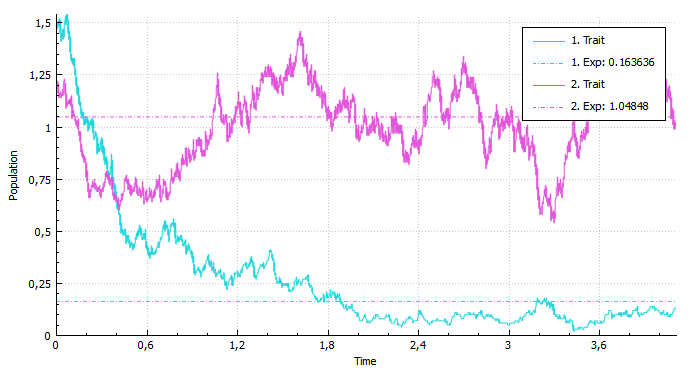
\includegraphics[width=1\linewidth]{./Pictures/LPANormalisierungK100}%
		\\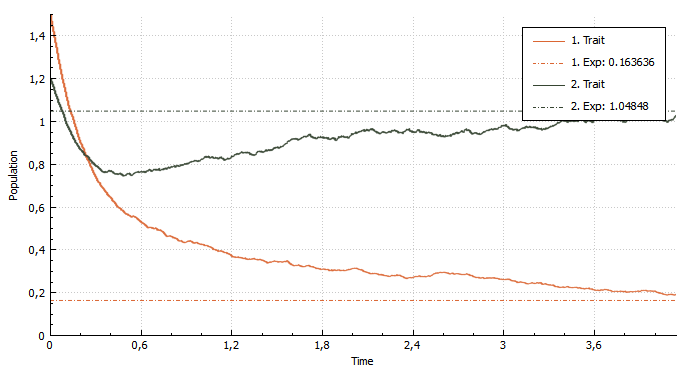
\includegraphics[width=1\linewidth]{./Pictures/LPANormalisierungK10000}%
		\end{figure}
	\end{minipage}
	\begin{minipage}{0.49\textwidth}
		Bsp. einer LPA-Normalisierung mit $ K = 100 \text{ und } K = 10000 $:
		\begin{itemize}
			\item Flacherer Verlauf der zeitlichen Entwicklung.\pause
			\item Einzelne Ereignisse lassen sich nicht mehr nachvollziehen.\pause
			\item Mit wachsendem K wird der Prozess zunehmend deterministisch und weicht immer weniger von anderen Simulationen ab.
		\end{itemize}
	\begin{center}
	\end{center}
	\end{minipage}\\
\end{frame}

\begin{frame}{Konvergenz}
	Tats"achlich konvergiert der Prozess mit $ K \to \infty $.
\end{frame}

\begin{frame}
	\frametitle{Gleichgewicht}
	Im stabilen Zustand ändert sich die Populationsgröße nicht mehr:
	\pause
	\begin{itemize}
		\item Für Monomorphe Population:
			\begin{align*}
			0 & = \dot{n} = (b(x) - d(x) - \bar{n}c(x,x))\bar{n}\\
			\bar{n}_x &= \frac{\left[ b(x)-d(x) \right]_+}{c(x,x)}
			\end{align*}
			\pause
		\item Für Dimorphe Population:
			\[ n_x = \frac{(b(x) - d(x))c(y,y)-(b(y)-d(y))c(x,y)}{c(y,y)c(x,x) - c(y,x)c(x,y)} \]
			oder $ (\bar{n}_x, 0)$, $ (0, \bar{n}_y)$ bzw. $ (0,0) $
	\end{itemize}
\end{frame}

\subsection{Fitness}
\begin{frame}
	\frametitle{Fitness-Funktion}
	\[ f(x,y) = b(x) - d(x) - c(x,y)\bar{n}_y \]\pause
	\begin{itemize}
		\item Sie gibt an wie gut sich ein Merkmal durchsetzten kann
		\item Asymptotische Wachstumsrate von y, wenn x im Zustand $ \bar{n}_x $ ist und y nur wenige Individuen hat
		\item Ermöglicht Aussagen über die Überlebenswahrscheinlichkeit einer Mutation
		\item Ermöglicht Aussagen über die angenommenen stabilen Zustände.
	\end{itemize}
	\pause
	Da wir nur eine Mutation zu den Nachbarn berücksichtigen, ist unsere Fitness Matrix eine Bandmatrix
\end{frame}

\begin{frame}{TSS-Prozesse}
	Ein besonderer Grenzwert Prozess ist der TSS-Prozess.
\end{frame}

\end{document}
% ä Ä ö Ö ü Ü